% Standalone TikZ figure: Teacher-Student Framework for Domain Adaptation
% For Chapter 6: Domain Adaptation and Sim-to-Real Transfer
\documentclass[tikz,border=10pt]{standalone}
\usepackage{tikz}
\usepackage{amsmath}
\usetikzlibrary{arrows.meta, positioning, shapes.geometric, fit, backgrounds, calc, patterns, decorations.pathreplacing}

\begin{document}
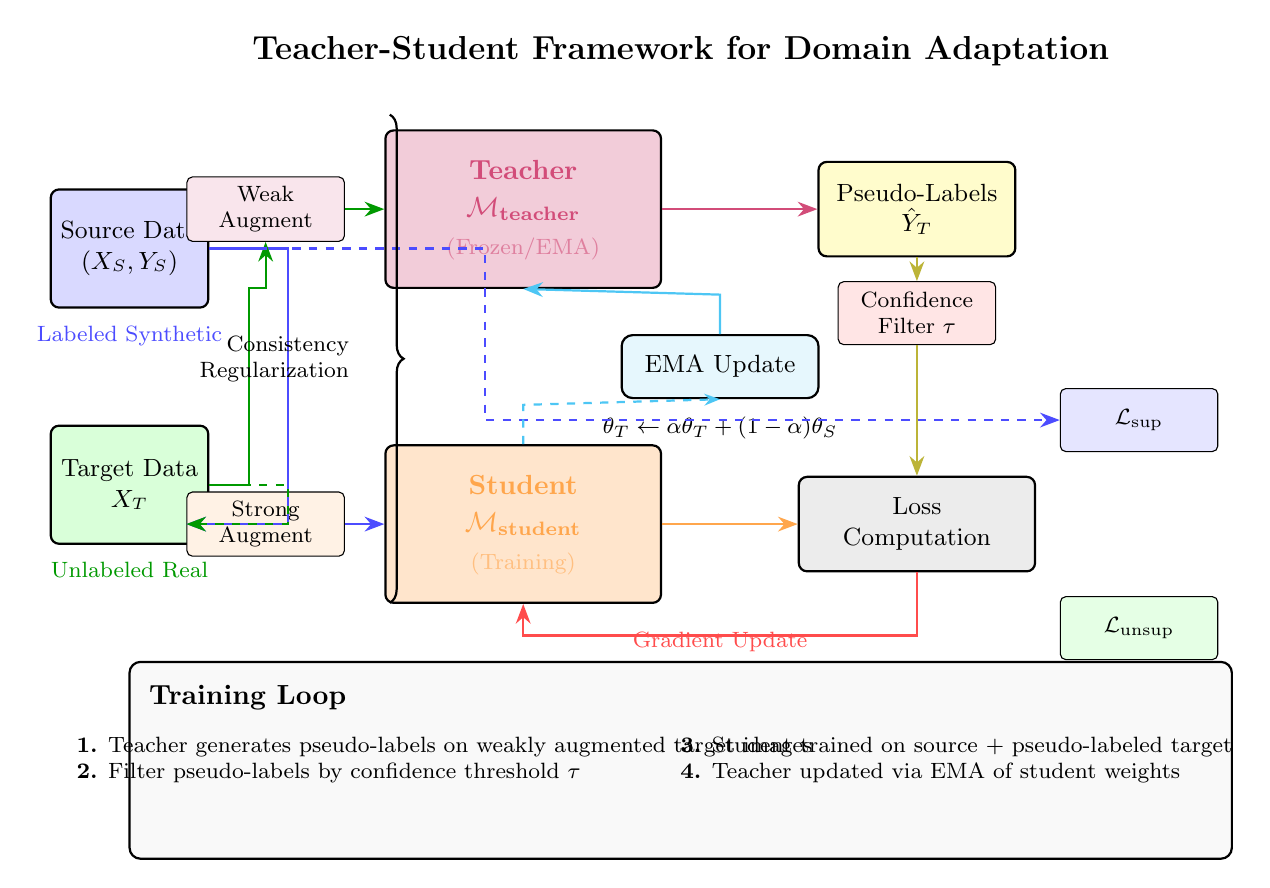
\begin{tikzpicture}[
    node distance=1cm and 1.5cm,
    every node/.style={font=\small},
    box/.style={rectangle, draw, thick, minimum width=2.5cm, minimum height=1.2cm, align=center, rounded corners=3pt},
    smallbox/.style={rectangle, draw, minimum width=2cm, minimum height=0.8cm, align=center, rounded corners=2pt, font=\footnotesize},
    databox/.style={rectangle, draw, thick, minimum width=2cm, minimum height=1.5cm, align=center, rounded corners=3pt},
    arrow/.style={-{Stealth[length=2.5mm]}, thick},
    darrow/.style={-{Stealth[length=2mm]}, thick, dashed},
    label/.style={font=\footnotesize}
]

% Title
\node[font=\bfseries\large] at (7, 6) {Teacher-Student Framework for Domain Adaptation};

% ============ DATA SOURCES ============
% Source (Synthetic) Data
\begin{scope}[shift={(0, 3.5)}]
    \node[databox, fill=blue!15] (srcdata) at (0, 0) {Source Data\\$(X_S, Y_S)$};
    \node[label, below=0.1cm of srcdata, text=blue!70] {Labeled Synthetic};
\end{scope}

% Target (Real) Data
\begin{scope}[shift={(0, 0.5)}]
    \node[databox, fill=green!15] (tgtdata) at (0, 0) {Target Data\\$X_T$};
    \node[label, below=0.1cm of tgtdata, text=green!60!black] {Unlabeled Real};
\end{scope}

% ============ TEACHER NETWORK ============
\begin{scope}[shift={(5, 4)}]
    \node[box, fill=purple!20, minimum width=3.5cm, minimum height=2cm] (teacher) at (0, 0) {};
    \node[font=\bfseries, purple!70] at (0, 0.5) {Teacher};
    \node[font=\bfseries, purple!70] at (0, 0) {$\mathcal{M}_{\text{teacher}}$};
    \node[label, purple!50] at (0, -0.5) {(Frozen/EMA)};

    % Weak augmentation indicator
    \node[smallbox, fill=purple!10, left=0.5cm of teacher] (weakaug) {Weak\\Augment};
\end{scope}

% ============ STUDENT NETWORK ============
\begin{scope}[shift={(5, 0)}]
    \node[box, fill=orange!20, minimum width=3.5cm, minimum height=2cm] (student) at (0, 0) {};
    \node[font=\bfseries, orange!70] at (0, 0.5) {Student};
    \node[font=\bfseries, orange!70] at (0, 0) {$\mathcal{M}_{\text{student}}$};
    \node[label, orange!50] at (0, -0.5) {(Training)};

    % Strong augmentation indicator
    \node[smallbox, fill=orange!10, left=0.5cm of student] (strongaug) {Strong\\Augment};
\end{scope}

% ============ PSEUDO-LABELS ============
\begin{scope}[shift={(10, 4)}]
    \node[box, fill=yellow!20] (pseudo) at (0, 0) {Pseudo-Labels\\$\hat{Y}_T$};
    \node[smallbox, fill=red!10, below=0.3cm of pseudo] (filter) {Confidence\\Filter $\tau$};
\end{scope}

% ============ LOSS COMPUTATION ============
\begin{scope}[shift={(10, 0)}]
    \node[box, fill=gray!15, minimum width=3cm] (loss) at (0, 0) {Loss\\Computation};

    % Loss components
    \node[smallbox, fill=blue!10, above right=0.3cm and 0.3cm of loss] (lsup) {$\mathcal{L}_{\text{sup}}$};
    \node[smallbox, fill=green!10, below right=0.3cm and 0.3cm of loss] (lunsup) {$\mathcal{L}_{\text{unsup}}$};
\end{scope}

% ============ EMA UPDATE ============
\begin{scope}[shift={(7.5, 2)}]
    \node[draw, thick, rounded corners, fill=cyan!10, minimum width=2.5cm, minimum height=0.8cm] (ema) {EMA Update};
    \node[label, below=0.1cm of ema] {$\theta_T \leftarrow \alpha\theta_T + (1-\alpha)\theta_S$};
\end{scope}

% ============ ARROWS AND CONNECTIONS ============
% Source data to student (supervised)
\draw[arrow, blue!70] (srcdata.east) -- ++(1,0) |- (strongaug.west);
\draw[arrow, blue!70] (strongaug.east) -- (student.west);

% Target data flow
\draw[arrow, green!60!black] (tgtdata.east) -- ++(0.5,0) -- ++(0, 2.5) -| (weakaug.south);
\draw[arrow, green!60!black] (weakaug.east) -- (teacher.west);

% Target data to student (through strong augment)
\draw[arrow, green!60!black, dashed] (tgtdata.east) -- ++(1,0) |- (strongaug.west);

% Teacher to pseudo-labels
\draw[arrow, purple!70] (teacher.east) -- (pseudo.west);

% Pseudo-labels through filter to loss
\draw[arrow, yellow!70!black] (pseudo.south) -- (filter.north);
\draw[arrow, yellow!70!black] (filter.south) -- ++(0, -0.5) -| (loss.north);

% Student outputs to loss
\draw[arrow, orange!70] (student.east) -- ++(0.5, 0) |- (loss.west);

% Source labels to supervised loss
\draw[arrow, blue!70, dashed] (srcdata.east) -- ++(3.5,0) |- (lsup.west);

% Loss to student (gradient)
\draw[arrow, red!70, thick] (loss.south) -- ++(0, -0.8) -| (student.south);
\node[label, red!70] at (7.5, -1.5) {Gradient Update};

% EMA connection
\draw[darrow, cyan!70, thick] (student.north) -- ++(0, 0.5) -- (ema.south);
\draw[arrow, cyan!70, thick] (ema.north) -- ++(0, 0.5) -- (teacher.south);

% ============ LEGEND / KEY STEPS ============
\begin{scope}[shift={(0, -3)}]
    \node[draw, thick, rounded corners, fill=gray!5, minimum width=14cm, minimum height=2.5cm] at (7, 0) {};
    \node[font=\bfseries] at (1.5, 0.8) {Training Loop};

    \node[font=\footnotesize, align=left] at (4, 0) {
        \textbf{1.} Teacher generates pseudo-labels on weakly augmented target images\\
        \textbf{2.} Filter pseudo-labels by confidence threshold $\tau$
    };
    \node[font=\footnotesize, align=left] at (10.5, 0) {
        \textbf{3.} Student trained on source + pseudo-labeled target\\
        \textbf{4.} Teacher updated via EMA of student weights
    };
\end{scope}

% ============ ANNOTATIONS ============
% Consistency regularization annotation
\draw[decorate, decoration={brace, amplitude=5pt, raise=3pt}, thick]
    (3.2, 5.2) -- (3.2, -1) node[midway, left=8pt, align=right, font=\footnotesize] {
        Consistency\\Regularization
    };

\end{tikzpicture}
\end{document}
